%% ID: bike_power
%% TITLE: Cycling Through Wind
%% TYPE: question
%% QUESTIONTYPE: numeric
%% CONCEPTS:  vectors, resolving_vectors, power
%% VIDEOS: 
%% LEVEL: 6
%% TOPIC: mechanics/dynamics
%% ORDER: 6

%\input{../../../Templates/Problem_Template}
%\begin{document}
\begin{problem}[Bike Power on a Windy Day] %A2-1
{A cyclist travels along a straight road at speed \vari{v} on two separate occasions; on Day 1 there is no wind, whereas on Day 2 there is a steady wind blowing at a speed \vari{w} in a direction perpendicular to the road (i.e. a cross-wind). The force on the cyclist due to air resistance is proportional to the square of the speed of the air relative to the cyclist; as a consequence, to maintain the same constant speed \vari{v} on Day 2 as on Day 1, the cyclist has to produce a greater power output. In what follows, assume that \valuedef{v}{20}{km h$^{-1}$} and \valuedef{w}{40}{km h$^{-1}$}
\begin{enumerate}
\item Draw diagrams showing the velocities of the cyclist and air in both the road frame and the cyclist’s frame of reference (i) on Day 1 when there is no wind and (ii) on Day 2 when there is the cross-wind. Hence find the speed of the air and the
direction in which it is moving relative to the cyclist when the steady cross-wind is blowing.
\item  Draw additional diagrams showing the velocity of the cyclist and the force due to air resistance on Day 1 and on Day 2. Hence deduce the factor by which the cyclist must increase power to maintain a constant speed in the cross-wind.
\end{enumerate}}
{\textit{From Julia Riley's 1A Dynamics Question Sheet}}
{\begin{enumerate}
\item 
If the direction of motion of the bike along the road is defined as being in the positiv  \vari{x} direction, in order to move into the cyclist's frame of reference from the road frame of reference, a velocity of magnitude \vari{v} in the negative \vari{x} direction must be added to the velocities of both the cyclist and the air. As expected, this gives an overall velocity of zero for the cyclist in their reference frame, as shown in Figure \ref{fig:dynamics_bike_air_velocities}.

\begin{figure}[h]
\centering
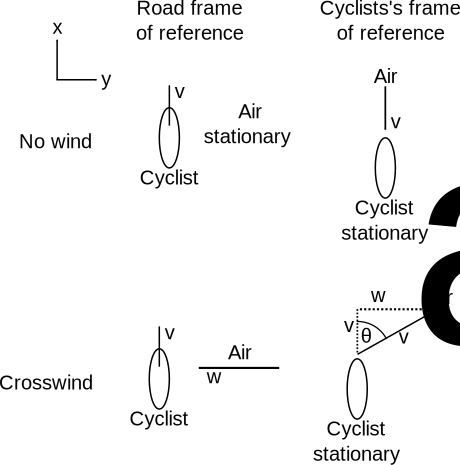
\includegraphics[scale =0.7]{../../../figures/dynamics_bike_air_velocities.svg}
\caption{}
\label{fig:dynamics_bike_air_velocities}
\end{figure}

On Day 2 the air speed in the cyclists's frame, \vari{v_{air}} is therefore given by $v_{air}^2 = v^2 + w^2$, giving \valuedef{v_{air}}{44.7}{km h$^{-1}$}. The angle \vari{\theta} between the direction of motion of the cyclist and the direction of the motion of the air is given by $\tan \theta = \frac{w}{v}$, giving \valuedef{\theta}{63.4}{$^{\circ}$}.

\item  The force due to air resistance acts on the cyclist in the same direction as the velocity of the air in the cyclist's reference frame, as shown in Figure \ref{fig:dynamics_bike_air_forces}.

\begin{figure}[h]
\centering
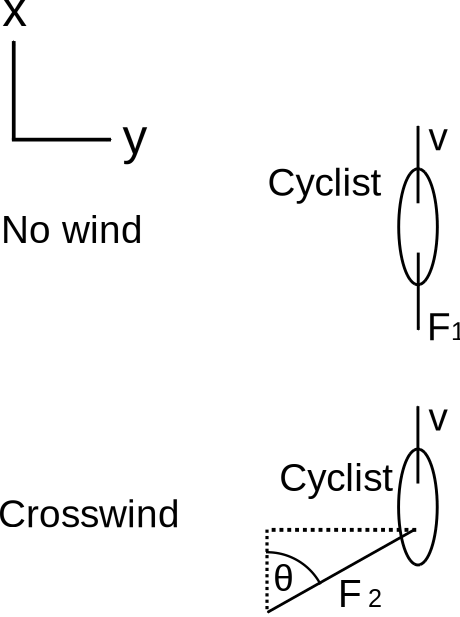
\includegraphics[scale =0.5]{../../../figures/dynamics_bike_air_forces.svg}
\caption{}
\label{fig:dynamics_bike_air_forces}
\end{figure}

On day 2, as the air resistance force acts along the direction of motion the power required for the cyclist to overcome this is given by $P_1 = F_1 . v$. As the force due to air resistance is proportional to the square of the speed of the air relative to the cyclists, \vari{F_1} can be written as $F_1 = k v^2$, giving $P_1 = k v^3$.

On Day 2, the air resistance force is $F_2 = k v_{air}^2 = k (v^2 + w^2)$. However, to find the power the cyclist needs to overcome this and maintain a constant velocity we must use the component of this force acting in the direction of the motion of the cyclist, in this case the  \vari{x} direction. $F_{2x} = k (v^2 + w^2) \cos \theta$. From Figure  \ref{fig:dynamics_bike_air_velocities}, $ \cos \theta = \frac{v}{\sqrt{v^2 + w^2}}$, and so 
\begin{equation} F_{2x} = k (v^2 + w^2) \frac{v}{\sqrt{v^2 + w^2}} = kv \sqrt{v^2 + w^2}  \end{equation}

This leads to $P_2 = F_{2x} v = kv^2 \sqrt{v^2 + w^2}$. The factor by which the cyclist must increase power on day 2 is therfore given by
\begin{equation} \frac{P_2}{P_1} = \frac{ kv^2 \sqrt{v^2 + w^2}}{k v^3} = \frac{ \sqrt{v^2 + w^2}}{ v}\end{equation}

Substituting in the numerical values for \vari{v} and \vari{w} gives  
\begin{equation}\frac{P_2}{P_1}= \frac{ \sqrt{20^2 + 40^2}}{20} = 2.2\end{equation}

\end{enumerate}
}
\end{problem}
%\end{document}


